\documentclass[letterpaper,11pt]{article}

\author{Jacob Thomas Errington}
\date{21 February 2017}
\title{Assignment \#3\\Formal verification -- COMP 525}

\usepackage[margin=2.0cm]{geometry}
\usepackage{amsmath,amssymb,amsthm}
\usepackage{tikz}
\usetikzlibrary{automata, graphs, arrows}

\newtheorem{prop}{Proposition}

\renewcommand{\thesection}{Question \arabic{section}}
\newcommand{\question}{\section}
\renewcommand{\complement}{\overline}
\newcommand{\eventually}{\lozenge}
\newcommand{\always}{\square}
\newcommand{\nmodels}{\nvDash}
\newcommand{\step}{\bigcirc}
\DeclareMathOperator{\untilOp}{\mathtt{U}}
\newcommand{\until}{\untilOp{}}

\begin{document}

\maketitle

\question{Writing $\omega$-regular expressions for B\"uchi automata}

The left automaton can be represented by
\begin{equation*}
    (A \Sigma^* A + C \Sigma^* C)^\omega
\end{equation*}

The right automaton can be represented by
\begin{equation*}
    (B + C)^* (A (BC)^* ( (BC)^\omega + BA^\omega ) + B A^\omega )
\end{equation*}

\question{Properties of DBAs}

\begin{prop}
    The class of DBAs is not closed under complementation.
\end{prop}

\begin{proof}
    To see this, we will find a DBA whose complement language cannot be
    recognized by a DBA. We know that the language represented by the
    $\omega$-regular expression $R = (A + B)^* B^\omega$ cannot be recognized
    by a DBA. Let $L(R)$ be the language recognized by an NBA represented by
    the expression $R$. In natural language, this language is the set of all
    strings with only finitely many $A$. Hence, if a string is \emph{not} in
    this language, then it has infinitely many $A$. Consequently, the
    complement language, in which $A$ appears infinitely many times,
    $\complement{L(R)}$ is recognized by an NBA represented by the
    $\omega$-regular expression $\complement{R} = (\Sigma^* A)^\omega$.

    We claim that there is a DBA represented by $\complement{R}$. Figure
    \ref{fig:dba} shows a deterministic automaton to recognize the language of
    the expression $\complement{R}$.

    However, $\complement{\complement{R}} = R$ is known to not be recognizable
    by a DBA. Hence, DBAs are not closed under complementation.

    \begin{figure}[ht]
        \begin{center}
            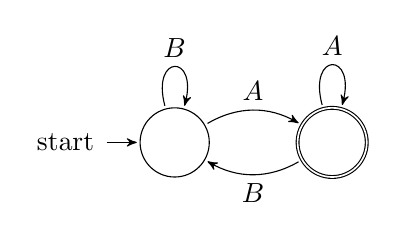
\begin{tikzpicture}[
                    node distance=2cm,
                    auto,
                    >=stealth',
                    shorten <=1pt,
                    shorten >=1pt,
                ]
                \node[state,initial] (s) {} ;
                \node[state,accepting,right of=s] (t) {} ;

                \graph[use existing nodes]{
                    s ->[loop above,edge label=$B$]
                    s ->[edge label=$A$,bend left=30]
                    t ->[loop above,edge label=$A$]
                    t ->[edge label=$B$,bend left=30]
                    s ;
                } ;
            \end{tikzpicture}
        \end{center}
        \caption{
            A DBA for the language of the expression $\complement{R}$.
        }
        \label{fig:dba}
    \end{figure}
\end{proof}

\question{Satisfying LTL formulas}

\begin{enumerate}
    \item $TS \nmodels \eventually \always c$

        Since after either start state, we reach infinite alternation between
        $s_4$ and one of $s_3, s_5, s_2$. In $s_4$, $c$ is false, whereas in
        each of $s_3, s_5, s_2$, $c$ is true. The infinite portion of any run
        through this automaton will have a strict alternation of $c$ being true
        and false. Consequently, we cannot have $\always c$ no matter how long
        we wait.

    \item $TS \models \always \eventually c$

        By the same argument about the infinite portion of the runs, $c$ occurs
        infinitely often.

    \item $TS \models \step \neg c \implies \step \step c$

        This deals just with the beginning of the string, and doesn't make any
        ``infinite claims''.
        This means we can exhaustively check the prefixes of relevant lengths.
        In particular, we have $\sigma_1 = s_1 s_3 s_4 \tau$,
        $\sigma_2 = s_1 s_4 \tau$, and $\sigma_3 = s_2 s_4 \tau$. Notice that
        in the first letter in $\tau$, $c$ is true (these are the states
        reachable in one step from $s_4$).

        $\sigma_1$ satisfies the property, since the premise of the implication
        is not satisfied, and from falsehood follows anything.
        $\sigma_2$ satisfies the property, since the premise is satisfied, and
        the first state in $\tau$ has $c$ true.
        $\sigma_3$ satisfies the property for the same reason.

    \item $TS \nmodels \always a$

        Any run starting in $s_2$ starts with $\neg a$, so those runs don't
        satisfy the property.

    \item $TS \models a \until \always (b \lor c)$

        In runs starting from $s_1$, we have $a$ true, and anywhere we go from
        there, we always have $b \lor c$ true.

        In runs starting from $s_2$, we don't have $a$. However, we have
        $b \lor c$ true right away. This is fine, because ``until'' allows the
        left hand side to possibly occur zero times.

    \item $TS \nmodels (\step \step b) \until (b \lor c)$

        Consider the run $\sigma = s_1 s_4 s_2 s_4 \tau$. It does reach a state
        where $b \lor c$ is true (namely $s_4$ right at the second letter), but
        it does not satisfy $\step \step b$ for all states leading up to that
        point. In particular, $\step \step b$ is not true of the initial state
        in this run.
\end{enumerate}

\end{document}
